\documentclass[border=5pt]{standalone}
\usepackage{fontspec}
\usepackage{unicode-math}
\setmainfont{Noto Serif}
\newfontfamily\FigureItalic{Noto Serif}
\setmathfont{STIXTwoMath-Regular.otf}
\usepackage{tikz}
\usetikzlibrary{arrows.meta,calc,patterns,decorations.pathmorphing,decorations.markings,decorations.pathreplacing,positioning,backgrounds}
\definecolor{Ink}{HTML}{000000}
\definecolor{Curve}{HTML}{000000}
\definecolor{Bzero}{HTML}{000000}
\definecolor{Bone}{HTML}{000000}
\definecolor{Btwo}{HTML}{000000}
\definecolor{Bthree}{HTML}{000000}
\definecolor{Bfour}{HTML}{000000}
\tikzset{
 ax/.style={draw=Ink,line width=.72pt,-{Latex[length=2.4mm,width=1.5mm]}},
 lev/.style={draw=Ink,line width=1.4pt,line cap=butt},
 thinlev/.style={draw=Ink,line width=.65pt,line cap=butt},
 helper/.style={draw=Ink,line width=.65pt},
 bare/.style={draw=Ink,line width=.95pt,dash pattern=on 4pt off 2.8pt},
 curve/.style={draw=Ink,line width=1.85pt,line cap=round,line join=round},
 ray/.style={draw=Ink,line width=1.0pt,-{Latex[length=2.3mm,width=1.4mm]}},
 measure/.style={draw=Ink,line width=.75pt,{Latex[length=1.9mm,width=1.2mm]}-{Latex[length=1.9mm,width=1.2mm]}},
 link/.style={draw=Ink,line width=1.0pt},
 wave/.style={draw=Ink,line width=.85pt,decorate,decoration={snake,amplitude=.33mm,segment length=2.5mm,pre length=.8mm,post length=.8mm}},
 photon/.style={draw=Ink,line width=1.0pt,-{Latex[length=2.0mm,width=1.3mm]},decorate,decoration={snake,amplitude=.4mm,segment length=2.7mm,pre length=0mm,post length=1.9mm}},
 lab/.style={text=Ink,font=\fontsize{13.5}{16}\selectfont,inner sep=2pt},
 small/.style={text=Ink,font=\fontsize{11.5}{14}\selectfont,inner sep=2pt},
 tag/.style={text=Ink,font=\fontsize{14}{17}\selectfont\FigureItalic\itshape,inner sep=2pt}}
\pagestyle{empty}

\begin{document}
% Figure 13.2; source-grounded revision.
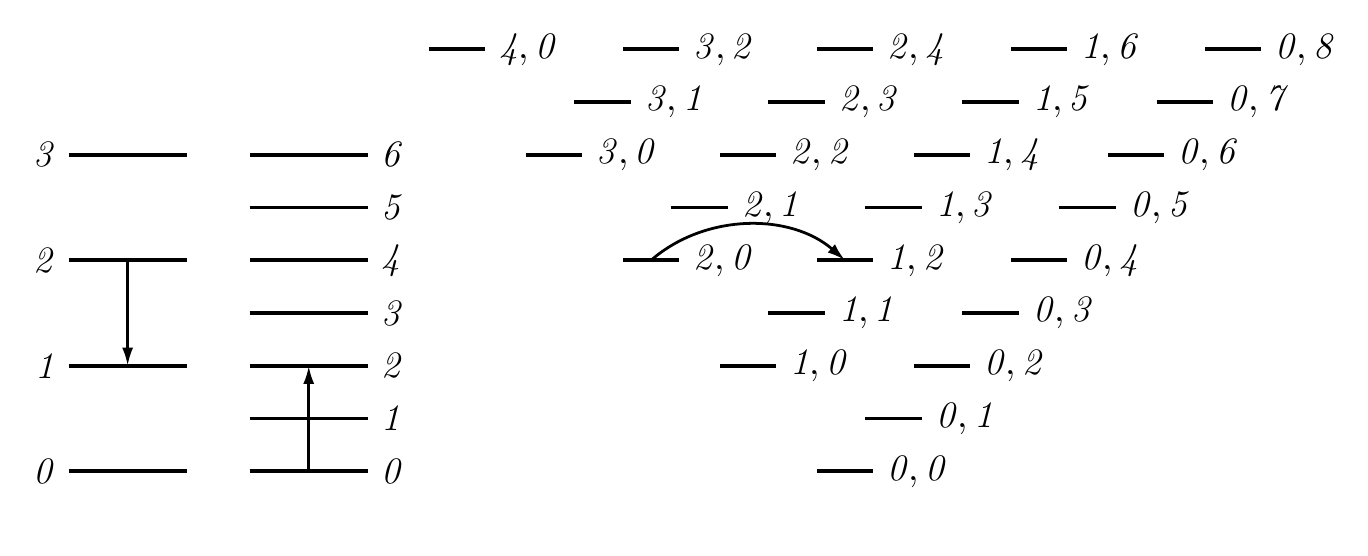
\begin{tikzpicture}[x=1cm,y=1cm]
\coordinate (h0) at (0.90000,0.00000);
\coordinate (h0L) at (0.15000,0.00000);
\coordinate (h0R) at (1.65000,0.00000);
\draw[lev] (h0L) -- (h0R);
\node[lab,anchor=east] at (0.05000,0.00000) {\textit{0}};
\coordinate (h1) at (0.90000,1.34000);
\coordinate (h1L) at (0.15000,1.34000);
\coordinate (h1R) at (1.65000,1.34000);
\draw[lev] (h1L) -- (h1R);
\node[lab,anchor=east] at (0.05000,1.34000) {\textit{1}};
\coordinate (h2) at (0.90000,2.68000);
\coordinate (h2L) at (0.15000,2.68000);
\coordinate (h2R) at (1.65000,2.68000);
\draw[lev] (h2L) -- (h2R);
\node[lab,anchor=east] at (0.05000,2.68000) {\textit{2}};
\coordinate (h3) at (0.90000,4.02000);
\coordinate (h3L) at (0.15000,4.02000);
\coordinate (h3R) at (1.65000,4.02000);
\draw[lev] (h3L) -- (h3R);
\node[lab,anchor=east] at (0.05000,4.02000) {\textit{3}};
\coordinate (l0) at (3.20000,0.00000);
\coordinate (l0L) at (2.45000,0.00000);
\coordinate (l0R) at (3.95000,0.00000);
\draw[lev] (l0L) -- (l0R);
\node[lab,anchor=west] at (4.05000,0.00000) {\textit{0}};
\coordinate (l1) at (3.20000,0.67000);
\coordinate (l1L) at (2.45000,0.67000);
\coordinate (l1R) at (3.95000,0.67000);
\draw[lev] (l1L) -- (l1R);
\node[lab,anchor=west] at (4.05000,0.67000) {\textit{1}};
\coordinate (l2) at (3.20000,1.34000);
\coordinate (l2L) at (2.45000,1.34000);
\coordinate (l2R) at (3.95000,1.34000);
\draw[lev] (l2L) -- (l2R);
\node[lab,anchor=west] at (4.05000,1.34000) {\textit{2}};
\coordinate (l3) at (3.20000,2.01000);
\coordinate (l3L) at (2.45000,2.01000);
\coordinate (l3R) at (3.95000,2.01000);
\draw[lev] (l3L) -- (l3R);
\node[lab,anchor=west] at (4.05000,2.01000) {\textit{3}};
\coordinate (l4) at (3.20000,2.68000);
\coordinate (l4L) at (2.45000,2.68000);
\coordinate (l4R) at (3.95000,2.68000);
\draw[lev] (l4L) -- (l4R);
\node[lab,anchor=west] at (4.05000,2.68000) {\textit{4}};
\coordinate (l5) at (3.20000,3.35000);
\coordinate (l5L) at (2.45000,3.35000);
\coordinate (l5R) at (3.95000,3.35000);
\draw[lev] (l5L) -- (l5R);
\node[lab,anchor=west] at (4.05000,3.35000) {\textit{5}};
\coordinate (l6) at (3.20000,4.02000);
\coordinate (l6L) at (2.45000,4.02000);
\coordinate (l6R) at (3.95000,4.02000);
\draw[lev] (l6L) -- (l6R);
\node[lab,anchor=west] at (4.05000,4.02000) {\textit{6}};
\draw[ray] (h2) -- (h1);
\draw[ray] (l0) -- (l2);
\node[tag] at (2.05000,-0.65000) {а};
% Q(a,b)=2a+b determines every ordinate, not manually staggered positions.
% The right panel is widened in x only to prevent labels merging into level bars.
\begin{scope}[xscale=1.10]
\coordinate (s0_0) at (9.10000,0.00000);
\coordinate (s0_0L) at (8.77500,0.00000);
\coordinate (s0_0R) at (9.42500,0.00000);
\draw[lev] (s0_0L) -- (s0_0R);
\node[lab,anchor=west] at (9.52500,0.00000) {$\mathit{0,0}$};
\coordinate (s0_1) at (9.66000,0.67000);
\coordinate (s0_1L) at (9.33500,0.67000);
\coordinate (s0_1R) at (9.98500,0.67000);
\draw[lev] (s0_1L) -- (s0_1R);
\node[lab,anchor=west] at (10.08500,0.67000) {$\mathit{0,1}$};
\coordinate (s1_0) at (7.98000,1.34000);
\coordinate (s1_0L) at (7.65500,1.34000);
\coordinate (s1_0R) at (8.30500,1.34000);
\draw[lev] (s1_0L) -- (s1_0R);
\node[lab,anchor=west] at (8.40500,1.34000) {$\mathit{1,0}$};
\coordinate (s0_2) at (10.22000,1.34000);
\coordinate (s0_2L) at (9.89500,1.34000);
\coordinate (s0_2R) at (10.54500,1.34000);
\draw[lev] (s0_2L) -- (s0_2R);
\node[lab,anchor=west] at (10.64500,1.34000) {$\mathit{0,2}$};
\coordinate (s1_1) at (8.54000,2.01000);
\coordinate (s1_1L) at (8.21500,2.01000);
\coordinate (s1_1R) at (8.86500,2.01000);
\draw[lev] (s1_1L) -- (s1_1R);
\node[lab,anchor=west] at (8.96500,2.01000) {$\mathit{1,1}$};
\coordinate (s0_3) at (10.78000,2.01000);
\coordinate (s0_3L) at (10.45500,2.01000);
\coordinate (s0_3R) at (11.10500,2.01000);
\draw[lev] (s0_3L) -- (s0_3R);
\node[lab,anchor=west] at (11.20500,2.01000) {$\mathit{0,3}$};
\coordinate (s2_0) at (6.86000,2.68000);
\coordinate (s2_0L) at (6.53500,2.68000);
\coordinate (s2_0R) at (7.18500,2.68000);
\draw[lev] (s2_0L) -- (s2_0R);
\node[lab,anchor=west] at (7.28500,2.68000) {$\mathit{2,0}$};
\coordinate (s1_2) at (9.10000,2.68000);
\coordinate (s1_2L) at (8.77500,2.68000);
\coordinate (s1_2R) at (9.42500,2.68000);
\draw[lev] (s1_2L) -- (s1_2R);
\node[lab,anchor=west] at (9.52500,2.68000) {$\mathit{1,2}$};
\coordinate (s0_4) at (11.34000,2.68000);
\coordinate (s0_4L) at (11.01500,2.68000);
\coordinate (s0_4R) at (11.66500,2.68000);
\draw[lev] (s0_4L) -- (s0_4R);
\node[lab,anchor=west] at (11.76500,2.68000) {$\mathit{0,4}$};
\coordinate (s2_1) at (7.42000,3.35000);
\coordinate (s2_1L) at (7.09500,3.35000);
\coordinate (s2_1R) at (7.74500,3.35000);
\draw[lev] (s2_1L) -- (s2_1R);
\node[lab,anchor=west] at (7.84500,3.35000) {$\mathit{2,1}$};
\coordinate (s1_3) at (9.66000,3.35000);
\coordinate (s1_3L) at (9.33500,3.35000);
\coordinate (s1_3R) at (9.98500,3.35000);
\draw[lev] (s1_3L) -- (s1_3R);
\node[lab,anchor=west] at (10.08500,3.35000) {$\mathit{1,3}$};
\coordinate (s0_5) at (11.90000,3.35000);
\coordinate (s0_5L) at (11.57500,3.35000);
\coordinate (s0_5R) at (12.22500,3.35000);
\draw[lev] (s0_5L) -- (s0_5R);
\node[lab,anchor=west] at (12.32500,3.35000) {$\mathit{0,5}$};
\coordinate (s3_0) at (5.74000,4.02000);
\coordinate (s3_0L) at (5.41500,4.02000);
\coordinate (s3_0R) at (6.06500,4.02000);
\draw[lev] (s3_0L) -- (s3_0R);
\node[lab,anchor=west] at (6.16500,4.02000) {$\mathit{3,0}$};
\coordinate (s2_2) at (7.98000,4.02000);
\coordinate (s2_2L) at (7.65500,4.02000);
\coordinate (s2_2R) at (8.30500,4.02000);
\draw[lev] (s2_2L) -- (s2_2R);
\node[lab,anchor=west] at (8.40500,4.02000) {$\mathit{2,2}$};
\coordinate (s1_4) at (10.22000,4.02000);
\coordinate (s1_4L) at (9.89500,4.02000);
\coordinate (s1_4R) at (10.54500,4.02000);
\draw[lev] (s1_4L) -- (s1_4R);
\node[lab,anchor=west] at (10.64500,4.02000) {$\mathit{1,4}$};
\coordinate (s0_6) at (12.46000,4.02000);
\coordinate (s0_6L) at (12.13500,4.02000);
\coordinate (s0_6R) at (12.78500,4.02000);
\draw[lev] (s0_6L) -- (s0_6R);
\node[lab,anchor=west] at (12.88500,4.02000) {$\mathit{0,6}$};
\coordinate (s3_1) at (6.30000,4.69000);
\coordinate (s3_1L) at (5.97500,4.69000);
\coordinate (s3_1R) at (6.62500,4.69000);
\draw[lev] (s3_1L) -- (s3_1R);
\node[lab,anchor=west] at (6.72500,4.69000) {$\mathit{3,1}$};
\coordinate (s2_3) at (8.54000,4.69000);
\coordinate (s2_3L) at (8.21500,4.69000);
\coordinate (s2_3R) at (8.86500,4.69000);
\draw[lev] (s2_3L) -- (s2_3R);
\node[lab,anchor=west] at (8.96500,4.69000) {$\mathit{2,3}$};
\coordinate (s1_5) at (10.78000,4.69000);
\coordinate (s1_5L) at (10.45500,4.69000);
\coordinate (s1_5R) at (11.10500,4.69000);
\draw[lev] (s1_5L) -- (s1_5R);
\node[lab,anchor=west] at (11.20500,4.69000) {$\mathit{1,5}$};
\coordinate (s0_7) at (13.02000,4.69000);
\coordinate (s0_7L) at (12.69500,4.69000);
\coordinate (s0_7R) at (13.34500,4.69000);
\draw[lev] (s0_7L) -- (s0_7R);
\node[lab,anchor=west] at (13.44500,4.69000) {$\mathit{0,7}$};
\coordinate (s4_0) at (4.62000,5.36000);
\coordinate (s4_0L) at (4.29500,5.36000);
\coordinate (s4_0R) at (4.94500,5.36000);
\draw[lev] (s4_0L) -- (s4_0R);
\node[lab,anchor=west] at (5.04500,5.36000) {$\mathit{4,0}$};
\coordinate (s3_2) at (6.86000,5.36000);
\coordinate (s3_2L) at (6.53500,5.36000);
\coordinate (s3_2R) at (7.18500,5.36000);
\draw[lev] (s3_2L) -- (s3_2R);
\node[lab,anchor=west] at (7.28500,5.36000) {$\mathit{3,2}$};
\coordinate (s2_4) at (9.10000,5.36000);
\coordinate (s2_4L) at (8.77500,5.36000);
\coordinate (s2_4R) at (9.42500,5.36000);
\draw[lev] (s2_4L) -- (s2_4R);
\node[lab,anchor=west] at (9.52500,5.36000) {$\mathit{2,4}$};
\coordinate (s1_6) at (11.34000,5.36000);
\coordinate (s1_6L) at (11.01500,5.36000);
\coordinate (s1_6R) at (11.66500,5.36000);
\draw[lev] (s1_6L) -- (s1_6R);
\node[lab,anchor=west] at (11.76500,5.36000) {$\mathit{1,6}$};
\coordinate (s0_8) at (13.58000,5.36000);
\coordinate (s0_8L) at (13.25500,5.36000);
\coordinate (s0_8R) at (13.90500,5.36000);
\draw[lev] (s0_8L) -- (s0_8R);
\node[lab,anchor=west] at (14.00500,5.36000) {$\mathit{0,8}$};
\draw[ray] (s2_0) .. controls (7.48720,3.28000) and (8.47280,3.28000) .. (s1_2);
\node[tag] at (9.65000,-0.65000) {б};
\end{scope}
\end{tikzpicture}

\end{document}
